%! TEX root = pre_konservasi.tex
% the main TeX file which is intended to compile, :VimtexReload after adjustment
   % this file should be included in the main file
% :h vimtex-tex-root
\documentclass[../rumukota.tex]{subfiles}
%ensure the class of docs

\begin{document}

\begin{figure}
	\begin{center}
		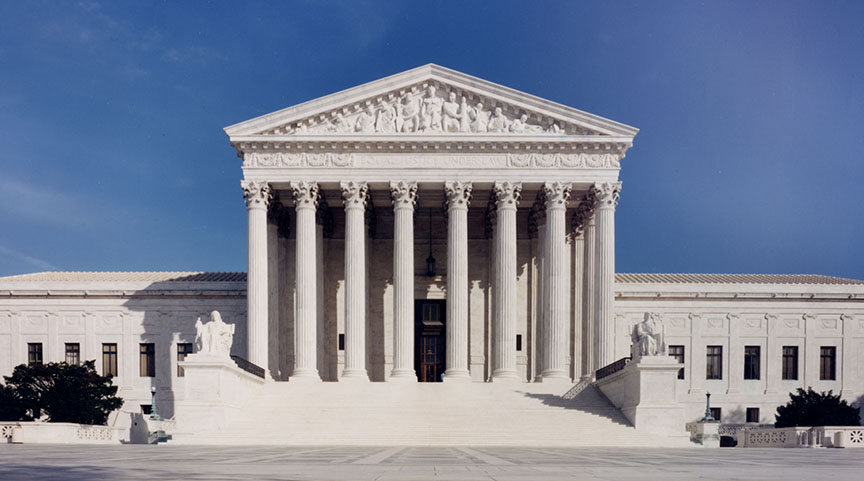
\includegraphics[width=.82\textwidth]{../figures/court_building.jpg}
		% filename may not contain space but _
	\end{center}
	\caption{SupremeCourt US}
	\label{fig:court}
\end{figure}

\begin{figure}
	\begin{center}
		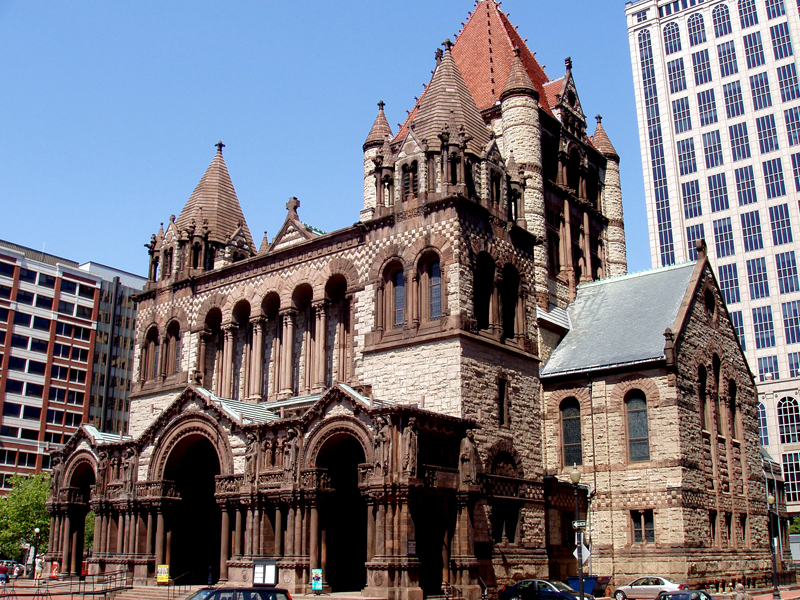
\includegraphics[width=.82\textwidth]{../figures/church_boston.jpg}
		% filename may not contain space but _
	\end{center}
	\caption{Geraja Boston}
	\label{fig:gerejaboston}
\end{figure}

\begin{figure}
	\begin{center}
		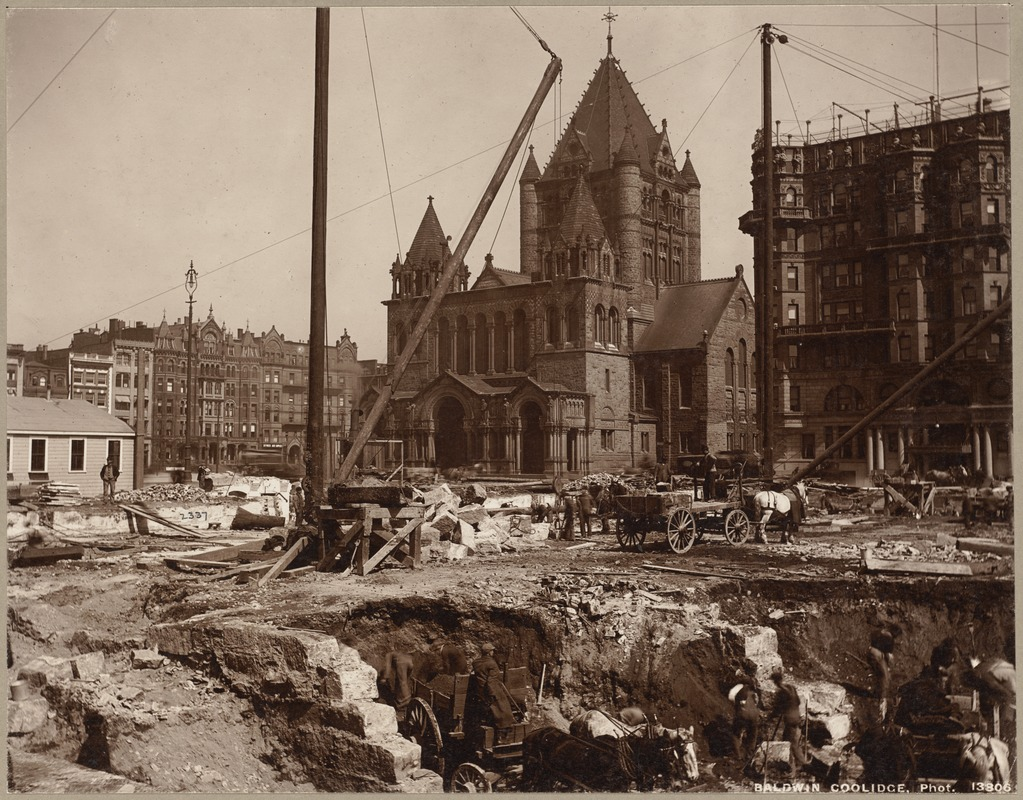
\includegraphics[width=.82\textwidth]{../figures/church_boston_old.jpg}
		% filename may not contain space but _
	\end{center}
	\caption{Geraja Boston Lama}
	\label{fig:gerejabostonlama}
\end{figure}






\bibliographystyle{apalike}
\bibliography{../filename.bib} % required for citecompletion, not work in mainfile
\end{document}

